\section{CVaR model}\label{sec:CVaR}

The CVaR model was built based on the first set of scenarios with start date 2008-02-27, obtained from scenario generaion chapter. 
Based on this set is determined the value and expected value of each ETF $i$, for each scenario $s$. In addition, is considered a initial budget of 1 million kr. 
The CVaR model is defined as
\begin{align}
\sum_{i} x_{i} &= \up{Budget} \\
\up{MeanReturn} &\ge \mu_{\up{Target}} \up{Budget} \\
\up{VaRDev}_{s} &\ge \up{Losses}_{s} - \up{VaR} \; \; \forall s \\
\up{Losses}_{s} &= \sum_{i} x_{i} - \sum_{i} \up{P}_{i,s} x_{i} \; \; \forall s \\
\up{CVaR} &= \up{VaR} + \frac{1} {1 - \alpha} \sum_{s} \up{pr}_{s} \up{VaRDev}_{s} \\
\up{MeanReturn} &= \sum_{i} \up{EP}_{i} x_{i}
\end{align}
where $ \mu_{\up{Target}}$ is 0, $\up{P}_{i,s}$ is the value of each ETF $i$ by scenario $s$, $\up{pr}_{s}$ is the probability of each scenario $s$ and is assumed to be linearly distributed over the scenarios, $\up{EP}_{i}$ is the expected value for each ETF $i$, and $\alpha$ is assumed to be 0.5.
In order to obtain the efficient frontier based on 10 optimal solutions of CVaR model is neccesary to find the minimum CVaR solution, as well as the CVaR solution related to the maximum possible return. 
Minimizing the model in order to CVaR variable, it returns the minimum CVaR solution of efficient frontier. 
Maximizing the model in order to MeanReturn variable, it returns the CVaR solution for the maximum average return. Based on this extreme points, a linear $\up{CVaR}_{\up{Target}}$ is created for the 10 runs. 
A constraint for limit the space solution movement to the $\up{CVaR}_{\up{Target}}$ is included in the CVaR model, and is defined as
\begin{align}
\up{CVaR} &\le \up{CVaR}_{\up{Target}} 
\end{align}
For each of the 10 runs, the CVaR model is optimized in order to maximize the MeanReturn variable. 
The efficient frontier of the 10 optimal solutions is presented in Figure~\ref{fig:frontier}. 

\begin{figure}[tp]
\centering
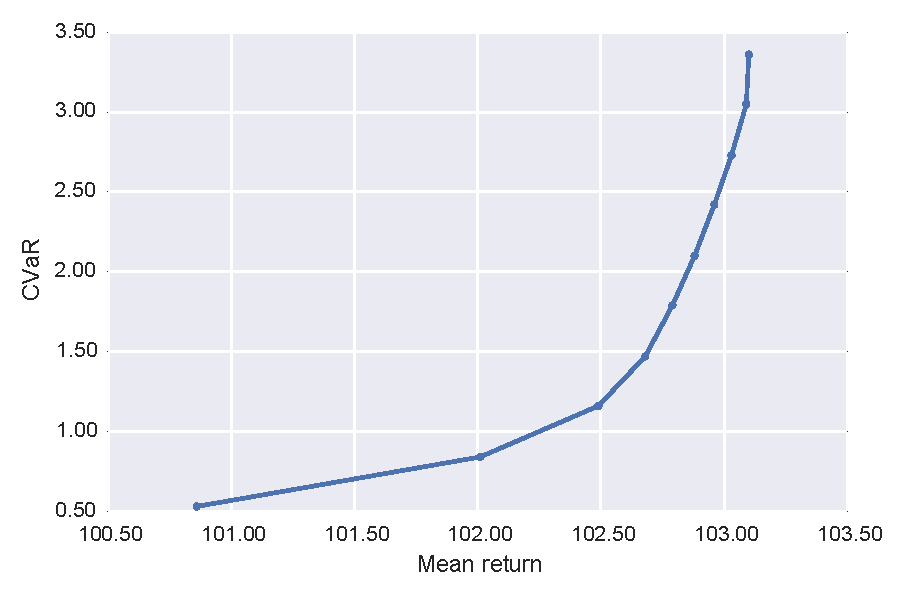
\includegraphics{../pic/frontier.pdf}
\caption{Optimal frontier for equidistant steps in CVaR.}
\label{fig:frontier}
\end{figure}

The portfolio results for each of the 10 runs is illustrated in Figure~\ref{fig:scenarioreturn}.
A CVaR bound of 0.0 indicates that CVaR is minimal, with 1.0 indicating that the optimization solely considers mean return.
One can see that FXI index increases its weight in the portfolio according to the increase of CVaR target. 
This happen because the increase of CVaR target leads to the maximization of return.
At that period (2008-02-27) of simulation, the scenario generation contain the historical of the last years, where FXI index leads to a higher return when compared to other indexs (as one can see in Figure~\ref{fig:prices_selected}). 

\begin{figure}[tp]
\centering
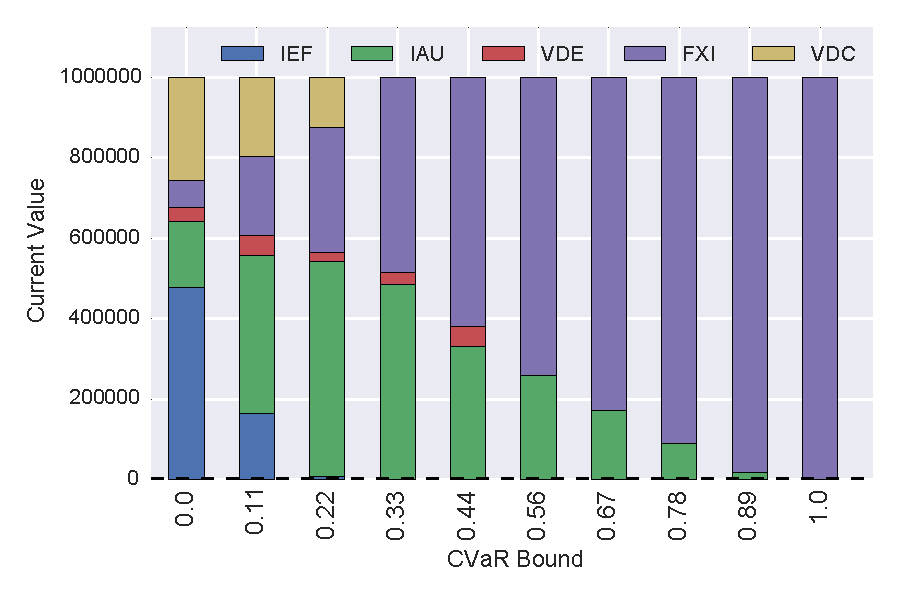
\includegraphics{../pic/Stake_vs_CVaR.pdf}
\caption{Portfolios at varying levels of the CVaR bound.}
\label{fig:scenarioreturn}
\end{figure}

Figure~\ref{fig:scenarioreturn} compares the scenario return at varying levels of the CVaR bound.
One can verify that the possibility of gettting higher return increase according to the increase of CVaR target  as expeceted.

\begin{figure}[tp]
\centering
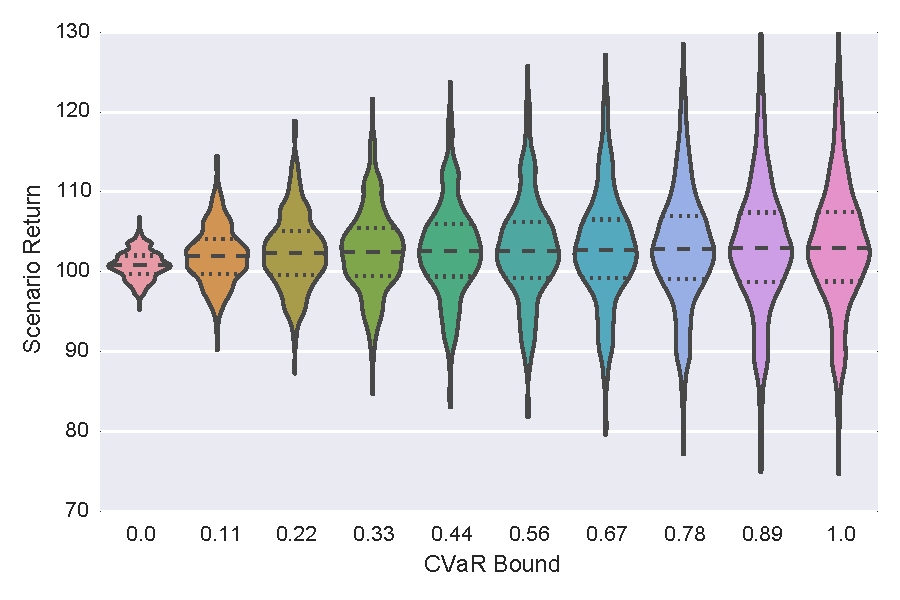
\includegraphics{../pic/Scenario_Return.pdf}
\caption{Scenario return for portfolios at varying levels of the CVaR bound.
The distributions for each bound are mirrored on the vertical axis, with the mean (dashed) and standard deviation (dotted) shown.}
\label{fig:scenarioreturn}
\end{figure}

